\subsection{Périmètres}

\prop{Formules calcul périmètre}
{Le périmètre d'un polygone se calcule en additionnant les longueurs de tous les côtés de la figure.}

\prop{Périmètre d'un cercle}
{Le périmètre d'un cercle de rayon $r$ se calcule avec la formule : $2\times \pi \times r$}

\subsubsection{Aires}

\begin{minipage}[t]{0.48\textwidth}
    \prop{Rectangle}
    {\begin{figure}[H]
        \centering
        \begin{tikzpicture}
            \draw (0,0)--(3,0) node[midway,above] {$L$} ;
            \draw (0,0)--(0,-2) node[midway,left] {$l$} ;
            \draw (0,-2)--(3,-2) ;
            \draw (3,-2)--(3,0) ;
        \end{tikzpicture}
        $$l\times L$$
    \end{figure}
    }
\end{minipage}
\hfill
\begin{minipage}[t]{0.48\textwidth}
    \prop{Carré}
    {\begin{figure}[H]
        \centering
        \begin{tikzpicture}
            \draw (0,0)--(2,0) node[midway,above,white] {$L$} ;%Pour alignement
            \draw (0,0)--(0,-2)node[midway,left] {$c$} ;
            \draw (0,-2)--(2,-2) ;
            \draw (2,-2)--(2,0) ;
        \end{tikzpicture}
        $$c\times c=c^2$$
    \end{figure}
    }
\end{minipage}

\begin{minipage}[t]{0.45\textwidth}
    \prop{Triangle}
    {\begin{multicols}{2}
        \begin{figure}[H]
            \centering
            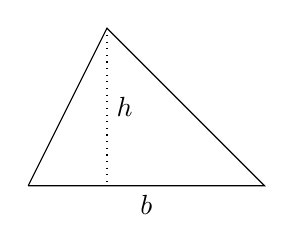
\begin{tikzpicture}
                \draw (0,0)--(1,2) --(3,0)--(0,0) node [midway, below] {$b$};
                \draw[dotted] (1,2)--(1,0) node [midway,right] {$h$};
                %\draw[dashed] (0,0) --(0,2)-- (3,2)--(3,0) ;
            \end{tikzpicture}
        \end{figure}
        \begin{figure}[H]
            \centering
            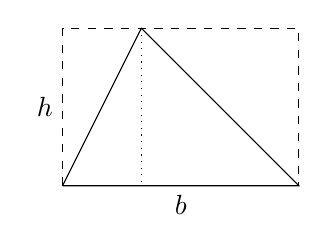
\begin{tikzpicture}
                \draw (0,0)--(1,2) --(3,0)--(0,0) node [midway, below] {$b$};
                \draw[dotted] (1,2)--(1,0);
                \draw[dashed] (0,0) --(0,2) node [midway,left ] {$h$} -- (3,2)--(3,0) ;
            \end{tikzpicture}
        \end{figure}
    \end{multicols}
    $$\dfrac{b\times h}{2}$$
    }
\end{minipage}
\hfill
\begin{minipage}[t]{0.55\textwidth}
    \prop{Losange}
    {\begin{multicols}{2}
        \begin{figure}[H]
            \centering
            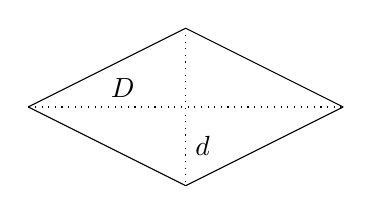
\begin{tikzpicture}
                \draw (0,0)--(2,1) node[midway,above,white] {$L$} ;%Pour alignement
                \draw (2,1)--(4,0);
                \draw [dotted] (0,0)--(4,0) ;
                \node at (1.2,0) [above] {$D$};
                \node at (2,-0.5) [right] {$d$};
                \draw [dotted] (2,1)--(2,-1) ;
                \draw (2,-1)--(4,0) ;
                \draw (2,-1)--(0,0) ;
            \end{tikzpicture}
        \end{figure}
        \begin{figure}[H]
            \centering
            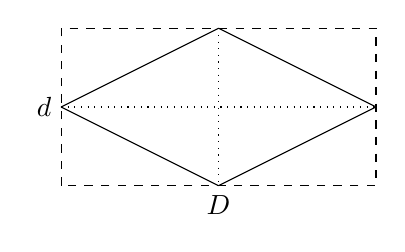
\begin{tikzpicture}
                \draw (0,0)--(2,1) node[midway,above,white] {$L$} ;%Pour alignement
                \draw (2,1)--(4,0);
                \draw [dotted] (0,0)--(4,0) ;
                \draw [dotted] (2,1)--(2,-1) ;
                \draw (2,-1)--(4,0) ;
                \draw (2,-1)--(0,0) ;
                \draw[dashed] (0,-1) -- (0,1) node[midway,left] {$d$}-- (4,1) --(4,-1) --(0,-1) node[midway,below] {$D$} ;
            \end{tikzpicture}
        \end{figure}
    \end{multicols}
    $$\dfrac{d\times D}{2}$$
    }
\end{minipage}


\begin{minipage}[t]{0.5\textwidth}
    \prop{Parallélogramme}
    {\begin{multicols}{2}
        \begin{figure}[H]
            \centering
            \begin{tikzpicture}[scale=0.9]
                \draw (-1,0)--(2,0) node[midway,above] {$b$} ;
                \draw (-1,0)--(0,-2);
                \draw[dotted] (1,0)--(1,-2)node[midway,left] {$h$} ;
                \draw (0,-2)--(3,-2) ;
                \draw (3,-2)--(2,0) ;
            \end{tikzpicture}
        \end{figure}
        \begin{figure}[H]
            \centering
            \begin{tikzpicture}[scale=0.9]
                \draw (-1,0)--(2,0) node[midway,above] {$b$} ;
                \draw (-1,0)--(0,-2);
                \draw[dotted] (1,0)--(1,-2);
                \draw[dashed] (2,0)--(2,-2);
                \draw[dashed] (-1,0)--(-1,-2) node[midway,left] {$h$} --(0,-2);
                \draw (0,-2)--(3,-2) ;
                \draw (3,-2)--(2,0) ;
            \end{tikzpicture}
        \end{figure}
    \end{multicols}
    \vspace{0.5em}
    $$b\times h$$
    }
\end{minipage}
\hfill
\begin{minipage}[t]{0.5\textwidth}
    \prop{Disque}
    {        \begin{figure}[H]
            \centering
            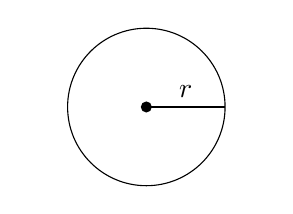
\begin{tikzpicture}
                \draw[white] (-1.5,0) rectangle (1.5,1);
                \draw (0,0) circle (1) ;
                \fill (0,0) coordinate (c) circle(2pt) ;
                \draw (0,0) -- (1,0) node[midway, above] {$r$};
            \end{tikzpicture}
        \end{figure}
    $$\pi \times r^2$$
    }
\end{minipage}

\subsection{Volumes}

\prop{Prisme}
{Pour un prisme, le volume se calcule avec la formule : $\text{Aire de la base}\times h$.}

\prop{Pyramide}
{Pour une pyramide, le volume se calcule avec la formule : $\dfrac{\text{Aire de la base}\times h}{3}$.}